\chapter{On Multimedia Analysis and Retrieval}
\epiquote{All our knowledge begins with the senses, proceeds then to the understanding, and ends with reason.}{Immanuel Kant}
\label{chapter:theory_multimedia_analysis_and_retrieval}

This chapter introduces the most important fundamentals on multimedia data, its analysis and the use of derivatives in information retrieval and processing systems. The main sources used in this chapter are the books \emph{Multimedia Retrieval} by H. Blanken et al \cite{Blanken:2007multimedia} and \emph{Similarity Search -- The Metric Space Approach} by P. Zezula et al. \cite{Zezula:2006similarity}, which both provide excellent introductions into the respective fields.

%\epiquote{Quote}{Author}
%%%%%%%%%%%%%%%%%%%%%%%%%%%%%%%%%%%%%%%%%%%%%%%%%%%%%%%%%%%%%%%%%%%%%%%%%%%%%%%%%%%%%

\section{Multimedia Data and Multimedia Collections}
\label{section:multmedia_data}

Multimedia data is ubiquitous and used in different forms in every area of our daily lives, be it private or professional. With the broad adoption of the smartphone in the early 2000s, almost every person on this planet now literally holds the tools required not only to consume but also produce multimedia content in the form of text, images, videos and audio snippets. Fueled by this technological progress, the past few decades have seen a staggering development in both \emph{volume} and \emph{variety} of multimedia data found in the wild, e.g., on the Internet or in personal or professional data collections. 

The term \emph{multimedia} refers to a combination of one or many different \emph{media types}, such as but not limited to, aural or visual information. We distinguish between these types, based on the representation we use when working and interacting with them. Sound, for example, is formed by airpressure waves that are registered by our ears. In contrast, visual information, involves electormagnetic waves captured by our eyes. In both cases, the brain plays an important role in interpreting the underlying processes and forming the human perception of the phenomenon. Similarily, we require different techniques when converting these media types from their analogue to their digital representation. We can roughly classify different media types based on their relationship with time. \emph{Static} media types (e.g., an image) do not exhibit a temporal development, wheras the information of \emph{dynamic} media types (e.g., an audio signal) depends on the time point that is being examined. \cite{Blanken:2007multimedia}

Traditionally, we often think of media as information that somehow can be perceived directly by our human senses. However, media data in a wider sense may also include less apparent examples such as motion capture data or data streams stemming from sensors or medical devices. 

Even though the various media types exhibit very different characteristics in their original representation, we find some commonalities once transfered into the digital domain. These shared properties are crucial for formalising the problem of processing and analysing such data in information processing systems in general and analytics and retrieval systems in particular.

\begin{description}
    \item[Analogue Correspondence] Most digital media types somehow reflect an analogue process taking place in the real-world. Converting such an analogue process to the digital domain requires several steps and intermediate representations, both digital and analogue (see Examples \ref{example:representation_visual_information} and \ref{example:representation_audio_information}).

    \item[Unstructured Data] The raw, digital representation of any media type is typically highly unstructured as opposed to, for example, the highly structured information found in a database. Consequently, we usually do not have natural units of information that can be leveraged directly for analysis. Therefore, information processing system rely on derivatives of the original data, gained through pre-processing and data analysis.
    
    \item[Semantic Gap] The derived representations of the original data usually highlight specific aspects thereof. Conversion between representations is therefore often accompanied by a loss of information, a problem often referred to as the \emph{semantic gap} \cite{Blanken:2007multimedia, Rossetto:2018thesis}.

    \item[Perceptive and Interpretative Gap] Reasoning about the content of any type of media, which is part of any analytical process, require several steps that involve preception and interpretation of the information by a human consumer. These processes are highly subjective and may lead to different results for different people, adding more indirection in addition to the semantic gap \cite{Rossetto:2018thesis}.
\end{description}

\begin{example}[label=example:representation_visual_information]{Digital Representation of Visual Information}{}
    \begin{wrapfigure}{L}{0.45\textwidth}
        \includegraphics[width=0.45\textwidth]{figures/example-visual-signal.eps}
    \end{wrapfigure}
    The visual information in a flat image is stored as a two dimensional array of \emph{pixels}. The information in every pixel is typically formed by a sensor, in an array of sensors, that captures the electormagnetic signal. Each pixel holds color values, usually one per color channel. For example, with the RGB color model, every pixel holds three values, one for the red, green and blue channel. The number of pixels per dimension determines the \emph{resolution} of the image. Typically, we use a fixed number of bits per colour -- the \emph{color depth} -- which determines the number colors that can be distinguished.

    If we take, for example, a coloured image of $1000 \times 1000$ pixel, we must encode \num{3e6} individual colour values. Using \SI{8}{\bit} per colour, we end up storing \SI{24e6}{\bit}, which amounts to \SI{3}{\mega\byte} worth of uncompressed image data. Images coming from modern cameras, exhibit resolutions much higher than that.
\end{example}

\begin{example}[label=example:representation_audio_information]{Digital Representation of Aural Information}{}
    \begin{wrapfigure}{R}{0.45\textwidth}
        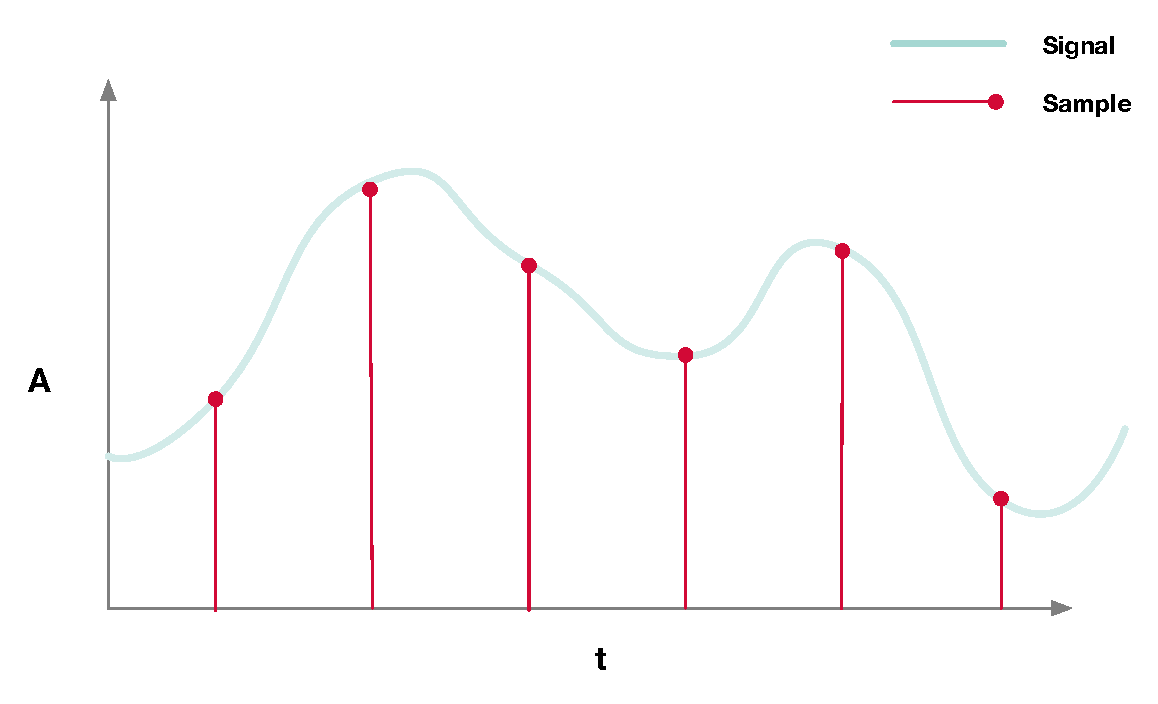
\includegraphics[width=0.45\textwidth]{figures/example-audio-signal.eps}
    \end{wrapfigure}
    The airpressure waves that form sound can be recorded and translated to an electrical signal by microphones. When digitizing this information, the amplitude of such a recorded audio signal is \emph{sampled} at a fixed rate. Each sample point consist of a value that quantizes the amplitude's energy at a given point in time to a number on a given range. An audio stream is then a sequence of these values. The quality of the process is determined by the \emph{sample rate}, i.e., the number of samples per time unit, and the \emph{bit depth}, which determines quantization of the amplitude power.

    If we take a \SI{1}{\second} audio snippet, sampled at \SI{44}{\kilo\hertz}, we end up storing \num{44000} sample points. Using a bit depth of \SI{16}{bit} per sample, this amounts to \SI{704000}{bit} or \SI{88}{\kilo\byte} of uncompressed audio data. In modern audio systems, we typically record multiple audio channels independently, leading to even more data.
\end{example}

\subsection{A Data Model for Media Data}

Despite being agnostic to the high-level data model in principle, the work in this Thesis still relies on an existing model for multimedia data due to its tight integration into the \emph{vitrivr} project \cite{Rossetto:2016vitrivr,Gasser:2019multimodal,Heller:2020multi}. This data model is illustrated in \Cref{figure:erm_mediadata_vitrivr} and enables organisation and management of media data in large collections as well as reasoning about the collection's content. In this model, a (multi-)media collection consists of multiple \emph{media object}s. The media object describes the data at the level of individual document -- e.g., a video or image file -- and comprises of basic attributes such its identifier, its media type or its path\footnote{The path forms the link to the raw media data in the filesystem, which we assume to be the most suited form of storage for this type of data.}. 

To account for the temporal development found in dynamic media types, the data model has a notion of a \emph{media segment}, which represents a clearly defined slice of the object and stands in a one-to-many relationship with it. The model does not make any explicit assumption as to how segments are formed. For static media types, such as images, there is a trivial one-to-one relationship between an object and a segment. For more complex media types, such as audio or video, \emph{media segmentation} is a dedicated area of research \cite{Koprinska:2001temporal} and can be approached in many different ways, e.g., at a fixed rate, based on changes in the content \cite{Foote:2000Automatic,Tsai:2016video} or using self-adaptive, deep neural networks~\cite{Souvcek:2019transnet}. Obiviously, different strategies for segmentation yield different degrees of summarization of information over time. The proposed model also allows for very application specific media types and segmentation strategies, such as \emph{image sequences} -- introduced for \acrshort{lsc} 2020 \cite{Heller:2020Interactive} -- which group related images per day for the purpose of lifelog analysis.

To model the different derivative representations that are used to describe a media object and its segments, the model foresees \emph{features}, which again stand in a one-to-many relationship to the segments. That is, every segment can have an arbitrary number of such features that describe different aspects of the segment's content. In practice, different types of features are obtained and stored in dedicated entities. Additionally, \emph{descriptive metadata} allows for a description of the media both at the document and segment level by means of simple key-value pairs containing descriptions or labels.

\begin{figure}[bt]
    \centering
    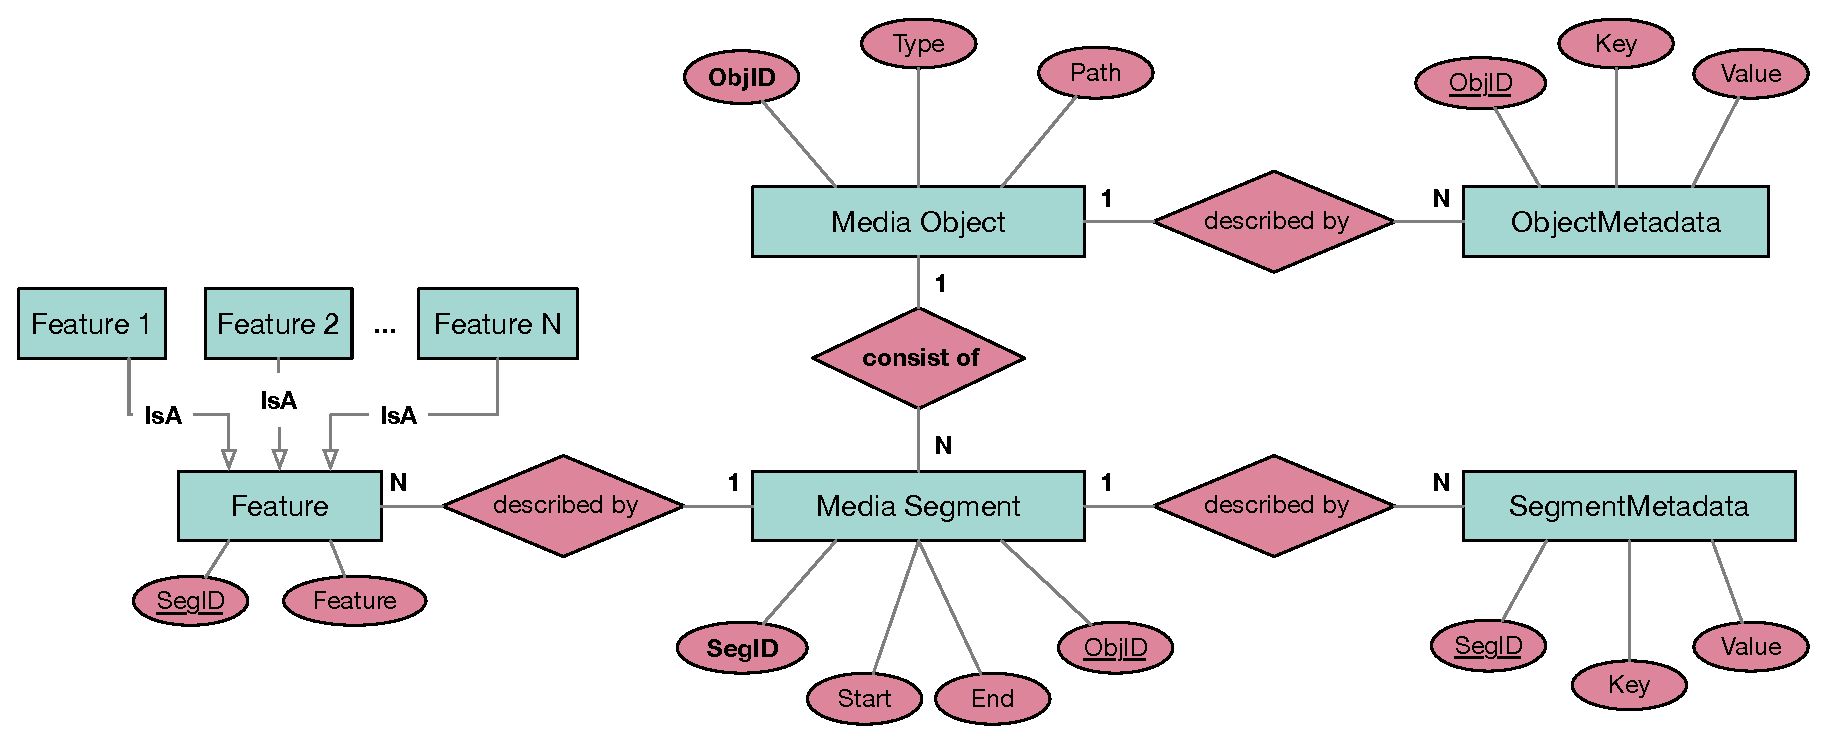
\includegraphics[width=\textwidth]{figures/erm-media-data-vitrivr}
    \caption{An extended \acrshort{erm} of the multimedia data model used in the \emph{vitrivr} project. The model is centered around the notion of media objects and media segments which are described by metadata and features.}
    \label{figure:erm_mediadata_vitrivr}
\end{figure}

While proven to be useful, the proposed model is only one possible approach to model media data and media collections and in  certain aspects, it stands in contrast to \cite{Blanken:2007multimedia}, which considers features to also be a type of metadata. 

For the purpose of this Thesis, we consider a slightly altered version of the aforementioned data model, which is more in line with \cite{Blanken:2007multimedia} and is illustrated in \Cref{figure:erm_mediadata}. It also considers media objects as abbstraction of individual files. However, this model foregoes the indirection introduced by the media segment and treats \emph{features}, \emph{annotations} and \emph{descriptions} as different types of a more general \emph{metadata} type that describes the media object directly. To model the temporal aspect in dynamic media types, the metadata itself exhibits information about the part of the object that is being described, denoted by an optional \emph{start} and an \emph{end} marker. In practice, this could be a frame number or a timestamp. 

While the difference between the two models may seem marginal, we argue, that the latter offers several advantages over the former: Firstly, it eliminates a level of indirection introduced by the media segment and thus simplifies handling of static media types, which are simply described by different types of metadata that lack a start and end marker. Secondly, it does not assume segmentation to be statically defined and instead makes this a property of the metadata itself. This is reasonable, because the optimal segmentation strategy may depend on a particular feature, especially when multiple media types must be considered jointly, e.g., sound and images in video. And finally, distinguishing between explicit types of metadata allows for optimisations at different levels of data organisation and management.

In reference to \cite{Blanken:2007multimedia}, one can roughly map a \emph{feature} in our proposed data model to a \emph{low-level} feature, whereas \emph{annotations} can be mapped to \emph{high-level} features. However, we do not fully agree with the proposed classification and will refrain from using it henceforth. 

\begin{figure}[bt]
    \centering
    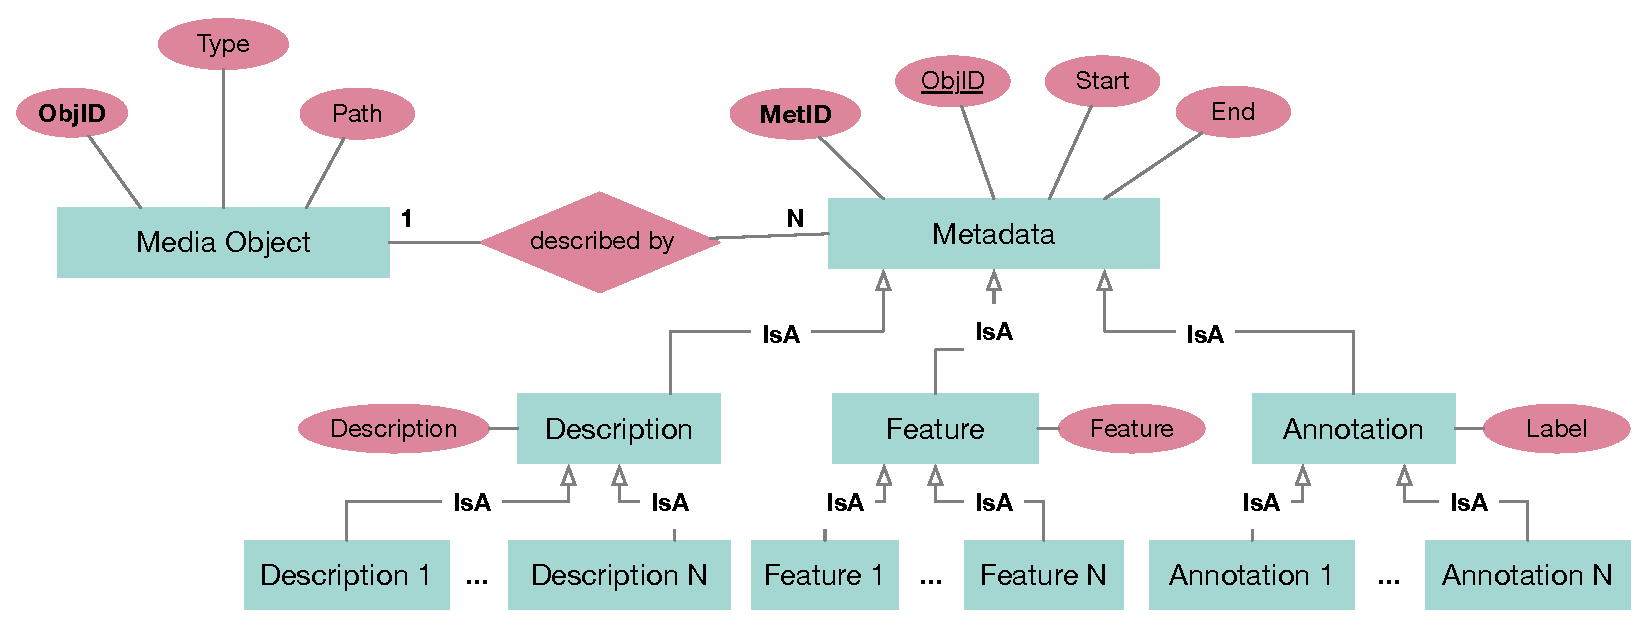
\includegraphics[width=\textwidth]{figures/erm-media-data}
    \caption{An extended \acrshort{erm} of the multimedia data model used in the \emph{vitrivr} project. The model is centered around the notion of media objects and media segments.}
    \label{figure:erm_mediadata}
\end{figure}

\subsubsection{Descriptive Metadata}
Descriptive metadata in the sense of the proposed data model comprises of textual descriptions (e.g, title, summary), technical information (e.g., duration, location, frame rate) and annotations (e.g., category labels). Such information has always played an important role in multimedia retrieval and analysis, because it provides (indirect) access to the media's content and can be leveraged in a structured way, e.g., in database queries. 

Over the years, many different metadata standards have emerged. For example, ID3\footnote{See https://id3.org/} tags allow for organisation of large music libraries and classification of songs based on information about artists or albums. Similarily, the Dublin Core Metadata Element Set (DCMES or just Dublin Core)\footnote{See https://www.dublincore.org/} comprises of 15 basic properties that can be used to describe any type of media, e.g., videos or images. And last but not least, EXIF\footnote{See https://www.loc.gov/preservation/digital/formats/fdd/fdd000146.shtml/} can be used to describe images and also includes technical metadata, such as the camera model, the exposure time or the f-number.

However, while useful and important for the problem of analysis and retrieval, this type of metadata comes with important disadvantages. Firstly, and notwithstanding recent developments in machine learning, e.g., in image captioning \cite{Hossain:2019Comprehensive}, such information is traditionally assigned manually in a laborious and time-consuming annotation process. This process is barely able to keep up with the ever increasing velocity at which new content is created. Secondly, descriptions and labels -- especially if not standardised -- are often subjective due to language, expertise and personal experience and may therefore differ depending on the person assigning them. This is closely related to the problem of the \emph{perceptive- and interpretative gap} \cite{Rossetto:2018thesis}. And finally, it is often challenging to describe the content of media in a textual manner, especially if temporal development is involved.\todo{We use this often. But is there some study on this?}

Regardless of these challenges, however, experience shows that annotations -- be they assigned manually or automatically -- play an important role, especially when it comes to information retrieval. A contributing factor here is that of query formulation, which is very low-effort ad familiar for textual information and becomes more challenging for other types of queries \todo{Source}.

\subsection{Features}
Simply put, a \emph{feature} is a mathematical object that captures ``derived characteristics''~\cite{Blanken:2007multimedia} of a media object or a segment thereof. A bit more formally, given a media collection $\mathcal{C}$, a \emph{feature} $f \in \mathcal{F}$ describes a temporal interval $[ \texttt{start}, \texttt{end} ]$ with $\texttt{start},\texttt{end} \in \symnatural_0$ of a media object $o \in \mathcal{C}$ under the feature transformation $\phi$, such that \Cref{eq:feature_transformation} holds.

\begin{equation}
    \label{eq:feature_transformation}
    \phi \colon \mathcal{C} \times \symnatural_0 \times \symnatural_0 \longrightarrow \mathcal{F}
\end{equation}

The process of generating features from media objects is called \emph{feature extraction} \cite{Blanken:2007multimedia} and there is an entire corpus of research that deals with the engineering of features and the feature extraction process for different media types. Usually, it involves the application of signal processing or statistical analysis techniques on the raw media data, which yields the relevant aspects of given media type's content, wherein ``relevant'' is very specific to the particular application or use-case. Various surveys, such as \cite{Ding:2012ASurvey,Salau:2019Feature}, cover the topic of feature extraction and we simply name and describe a few selected examples to provide an overview. An important point we would like to make here, however, is that there is no single feature that can be used to solve all types of problems.

For images, one can roughly distinguish between (low-level) colour, texture and shape features \cite{Salau:2019Feature}, as well as higher-level object- and keypoint detection features. An example of a colour feature could be a simple colour histogram or statistical moments that capture colour distributions, e.g., the average colour in a defined area of the image. Prominent examples for high-level features include algorithms such as \acrfull{sift}~\cite{Lowe:1999object} and \acrfull{surf}~\cite{Bay:2006surf} for keypoint and \acrfull{hog}~\cite{Dalal:2005Histograms} for object detection.
 

In practice, features are often real-valued vectors in a high-dimensional, real-valued vector space, i.e., $\mathcal{F} \subset \symreal^d$. 


Irrespective of their form, however, they can be anything that tries to find and capture patterns in the underlying data. Examples range from simple \emph{colour histograms} of images to \emph{statistical moments}. Feature modeling and generation, again, is a dedicated field of research for the different media types and over the decade, 


With the recent advances in machine learning and especially with the conception of the \emph{Convolutional Neural Network} for images, the process of feature extraction could be automated in that instead of engineering specific algorithms for finding pattern in data, neural networks learn to find these patterns themselves. Furthermore, these neural networks are now able to map the low-level features to higher-level concepts, thus bridging the semantic gap betwee what \cite{Blanken:2007multimedia} refers to as \emph{low-level and high-level features}.

\section{Multimedia Retrieval}

The research of domain of \emph{multimedia retrieval} deals with algorithms, methods and systems that allow for searching and obtaining items of interest from large multimedia collections. Many different subdomains for the different types of media have emerged over the years, including but not limited to image retrieval, \acrfull{mir} \cite{Simonetta:2019Multimodal}, video retrieval or 3D model retrieval.

\subsection{Similarity Search and the Vector Space Model}

In multimedia retrieval, there are two important assumptions for similiarity search. These assumptions can be summarized as follows:

\begin{itemize}
    \item For every object $c_{i}$ in a (multimedia) collection $\mathcal{C}$, there exists a feature transformation $\phi \colon \mathcal{C} \to \mathcal{F}$, that maps the object $o_{i} \in \mathcal{C}$ to a feature space $\mathcal{F}$.
    \item The feature space $\mathcal{F}$ and a to be defined distance function $\delta \colon \mathcal{F} \times \mathcal{F} \to \mathbb{R}_{\geq 0}$, constitute a metric space $(\mathcal{F},\delta)$, thus satisfying the non-negativity, identity of indiscernibles, symmetry and subadditivity condition.
\end{itemize}

The output of $\delta$ -- i.e., the calculated distance $d$ -- acts as a proxy for (dis-)similiarty between two objects $o_{i}$, $o_{j} \in \mathcal{C}$ given the feature transformation $\phi$. Hence, the closer two objects $o_{i}$, $o_{j}$ appear under the transformation, the more (dis-)similar they are. For the sake of completeness, it must be pointed out, that whether similarity is directly or inversely proportional to the distance is a matter of definition and depends on the concrete application. Also, in practice, multiple feature transformations $\phi_m$ may exist for a given media collection, leading to different feature spaces $\mathcal{F}_m$ for a collection $\mathcal{C}$ that must be considered jointly. Both aspects are usually addressed by additional \emph{correspondence} and \emph{scoring} functions.

\todo[inline]{Correspondence and score functions, score fusion}

\subsection{Approximate Nearest Neighbor Search}
The nearest neighbor search problem 

\todo[inline]{Describe techniques for approximate nearest neighbor search (ANN). Focus on a more conceptual overview of the types of algorithms rather than just enumerating concrete examples; this can be used as a build-up for discussing properties of different index structures later. }


\subsection{Beyond Similarity Search}
\todo[inline]{Retrieval and analytics techniques that go beyond simple similarity search (e.g. SOM, summarization, clustering)}

\section{Online Multimedia Analysis}
\todo[inline]{Introducing an online analysis pipeline (e.g., Pythia / Delphi).}

\section{Multimedia Analytics}
\todo[inline]{Describe how the combination of analysis }

\subsection{Beyond Similarity Search}

